\documentclass{article}

\usepackage{arxiv}

\usepackage[utf8]{inputenc} % allow utf-8 input
\usepackage[T1]{fontenc}    % use 8-bit T1 fonts
\usepackage{lmodern}        % https://github.com/rstudio/rticles/issues/343
\usepackage{hyperref}       % hyperlinks
\usepackage{url}            % simple URL typesetting
\usepackage{booktabs}       % professional-quality tables
\usepackage{amsfonts}       % blackboard math symbols
\usepackage{nicefrac}       % compact symbols for 1/2, etc.
\usepackage{microtype}      % microtypography
\usepackage{lipsum}
\usepackage{graphicx}

\title{Vaccinating Australia: How long will it take?}

\author{
    Mark Hanly
   \\
    Centre for Big Data Research in Health \\
    UNSW Sydney \\
  Sydney 2052 \\
  \texttt{\href{mailto:m.hanly@unsw.edu.au}{\nolinkurl{m.hanly@unsw.edu.au}}} \\
   \And
    Tim Churches
   \\
    Ingham Institute for Applied Medical Research \\
    South Western Sydney Clinical School, Faculty of Medicine, UNSW Sydney \\
  Liverpool \\
  \texttt{\href{mailto:timothy.churches@unsw.edu.au}{\nolinkurl{timothy.churches@unsw.edu.au}}} \\
   \And
    Oisín Fitzgerald
   \\
    Centre for Big Data Research in Health \\
    UNSW Sydney \\
  Sydney 2052 \\
  \texttt{\href{mailto:o.fitzgerald@unsw.edu.au}{\nolinkurl{o.fitzgerald@unsw.edu.au}}} \\
   \And
    Louisa Jorm
   \\
    Centre for Big Data Research in Health \\
    UNSW Sydney \\
  Sydney 2052 \\
  \texttt{\href{mailto:l.jorm@unsw.edu.au}{\nolinkurl{l.jorm@unsw.edu.au}}} \\
  }


% Pandoc citation processing

\usepackage{booktabs}
\usepackage{longtable}
\usepackage{array}
\usepackage{multirow}
\usepackage{wrapfig}
\usepackage{float}
\usepackage{colortbl}
\usepackage{pdflscape}
\usepackage{tabu}
\usepackage{threeparttable}
\usepackage{threeparttablex}
\usepackage[normalem]{ulem}
\usepackage{makecell}
\usepackage{xcolor}


\begin{document}
\maketitle

\def\tightlist{}


\begin{abstract}
Enter the text of your abstract here.
\end{abstract}

\keywords{
    COVID19
   \and
    vaccination
  }

\hypertarget{introduction}{%
\section{Introduction}\label{introduction}}

\begin{itemize}
\tightlist
\item
  Internationally, COVID19 continues to have devastating health and
  economic impacts.
\item
  In Australia, we have escaped much of the worst of the health impacts,
  through a combination of border closures, lock down measures and
  effective track and trace.
\item
  However this has come at a massive cost for many industries, including
  tourism, airlines, retails, the arts , international students etc.
\item
  A safe and effective vaccine is the best bet to return to normal.
\item
  Several viable vaccines have been developed or are close to
  completion, and Israel, The US and the UK have already begun to roll
  out national vaccination programs.
\item
  The Australian government has procured the Phizer and Astra-Zeneca
  vaccines (others?) and have released a national rollout strategy.
\item
  This strategy identifies 16 populations groups, ranked in priority
  across five vaccination phases (see Table 1).
\item
  Hospital hubs with cold chain storage facilities will administer the
  Phizer vaccine to the highest priority groups scheduled in Phase 1a.
\item
  Target of 80,000 vaccinations a day.
\item
  A back of the envelope calculation would suggest it would take 500
  days to vaccinate 20 million adult Australians twice.
\item
  But there are some complications e.g.~timing of second doses and
  vaccine hesitancy; we are going to need a bigger envelope.
\item
  Aim of this analysis is to calculate how long it will take the
  vaccinate the whole Australian population
\end{itemize}

\begin{table}[H]

\begin{threeparttable}
\caption{\label{tab:unnamed-chunk-1}Australia’s COVID-19 vaccine national roll-out strategy}
\centering
\begin{tabular}[t]{>{\raggedright\arraybackslash}p{1cm}>{\raggedright\arraybackslash}p{11cm}>{\raggedleft\arraybackslash}p{2cm}}
\toprule
Phase & Description & Size\\
\midrule
\textbf{\cellcolor{gray!6}{1a1}} & \cellcolor{gray!6}{Quarantine \& border workers} & \cellcolor{gray!6}{70,000}\\
\textbf{1a2} & Frontline health care workers & 100,000\\
\textbf{\cellcolor{gray!6}{1a3}} & \cellcolor{gray!6}{Aged care and disability care staff} & \cellcolor{gray!6}{318,000}\\
\textbf{1a4} & Aged care and disability care residents & 190,000\\
\textbf{\cellcolor{gray!6}{1b1}} & \cellcolor{gray!6}{Elderly adults aged 80 years and over} & \cellcolor{gray!6}{1,045,000}\\
\textbf{1b2} & Elderly adults aged 70-79 years & 1,858,000\\
\textbf{\cellcolor{gray!6}{1b3}} & \cellcolor{gray!6}{Other health care workers} & \cellcolor{gray!6}{953,000}\\
\textbf{1b4} & Aboriginal and Torres Strait Islander people aged 55 years and over & 87,000\\
\textbf{\cellcolor{gray!6}{1b5}} & \cellcolor{gray!6}{Younger adults with an underlying medical condition} & \cellcolor{gray!6}{2,000,000}\\
\textbf{1b6} & Critical and high risk workers & 196,000\\
\textbf{\cellcolor{gray!6}{2a1}} & \cellcolor{gray!6}{Adults aged 60-69} & \cellcolor{gray!6}{2,650,000}\\
\textbf{2a2} & Adults aged 50-59 & 3,080,000\\
\textbf{\cellcolor{gray!6}{2a3}} & \cellcolor{gray!6}{Aboriginal and Torres Strait Islander people aged 18-54} & \cellcolor{gray!6}{387,000}\\
\textbf{2a4} & Other critical and high risk workers & 453,000\\
\textbf{\cellcolor{gray!6}{2b}} & \cellcolor{gray!6}{Balance of adult population} & \cellcolor{gray!6}{6,643,000}\\
\textbf{3} & <18 if recommended & 5,670,000\\
\bottomrule
\end{tabular}
\begin{tablenotes}
\small
\item [] Adapted from https://www.health.gov.au/sites/default/files/documents/2021/01/australia-s-covid-19-vaccine-national-roll-out-strategy.pdf
\end{tablenotes}
\end{threeparttable}
\end{table}

\hypertarget{methods}{%
\section{Methods}\label{methods}}

\begin{itemize}
\tightlist
\item
  Vary three factors with two levels each resulting in 8 scenarios (see
  Table 2)
\item
  Daily vaccination capacity (60,000 versus 80,000)
\item
  Timing between first and second dose (3 to 6 weeks, versus 3 to 12
  weeks)
\item
  Vaccine hesitancy (7\% versus 13\%) based on recent survey data from
  Edwards et al (the projections assume taht hesitancy applies to
  general population groups but not to health or border workers, age
  care residents or those with an underlying condition)
\item
  Assume that the vaccine is administered according to the priority
  phases set out by the government
\item
  All groups within a given phase are given equal priority
\item
  Daily capacity is first divided between those needing second dose to
  ensure all second doses are delivered within the specified window; the
  remainder of the daily capacity distributed among those requiring
  their first dose.
\end{itemize}

\begin{table}[H]

\caption{\label{tab:unnamed-chunk-2}Projection scenarios}
\centering
\begin{tabu} to \linewidth {>{}l>{\raggedleft}X>{\raggedleft}X>{\raggedleft}X}
\toprule
Scenario & Capacity (units per day) & Gap between doses & Hesitancy\\
\midrule
\textbf{\cellcolor{gray!6}{1}} & \cellcolor{gray!6}{80,000} & \cellcolor{gray!6}{3 to 6 weeks} & \cellcolor{gray!6}{7\%}\\
\textbf{2} & 80,000 & 3 to 6 weeks & 13\%\\
\textbf{\cellcolor{gray!6}{3}} & \cellcolor{gray!6}{80,000} & \cellcolor{gray!6}{3 to 12 weeks} & \cellcolor{gray!6}{7\%}\\
\textbf{4} & 80,000 & 3 to 12 weeks & 13\%\\
\textbf{\cellcolor{gray!6}{5}} & \cellcolor{gray!6}{60,000} & \cellcolor{gray!6}{3 to 6 weeks} & \cellcolor{gray!6}{7\%}\\
\textbf{6} & 60,000 & 3 to 6 weeks & 13\%\\
\textbf{\cellcolor{gray!6}{7}} & \cellcolor{gray!6}{60,000} & \cellcolor{gray!6}{3 to 12 weeks} & \cellcolor{gray!6}{7\%}\\
\textbf{8} & 60,000 & 3 to 12 weeks & 13\%\\
\bottomrule
\end{tabu}
\end{table}

\hypertarget{results}{%
\section{Results}\label{results}}

\begin{itemize}
\item
  Under the most optimistic Scenario (Scenario 1), assuming vaccination
  starts on March 1, the highest priority group would be fully
  vaccinated with two doses by April 16th, just over six weeks (see
  Table 4).
\item
  However it would still take nearly nine months to complete Phase 2a,
  which includes adults aged 60-69 years.
\item
  It would take until July 2022 to fully vaccinate the adult population
  and a further four months after that to vaccinate those under 18.
\item
  Under this scenario, we would reach 50\% population coverage in
  February 2022 and 75\% population coverage in July 2022 (See Figure
  1A)
\item
  Under less optimistic scenarios it would take until the end of 2022 to
  vaccinate the adult population. (see Table 4)
\item
  Under this scenario, we would reach 50\% population coverage in May
  2022 and 75\% population coverage in December 2022 (See Figure 1B)
\end{itemize}

\begin{table}[H]

\caption{\label{tab:unnamed-chunk-3}Summary of vaccine rollout projects for different scenarios}
\centering
\begin{tabu} to \linewidth {>{}l>{\raggedleft}X>{\raggedleft}X>{\raggedleft}X>{\raggedright}X>{\raggedleft}X>{\raggedleft}X>{\raggedleft}X>{\raggedright}X}
\toprule
Scenario & Number of vaccinations & Individuals vaccinated & Population coverage & Phase 1a complete & Phase 1b complete & Phase 2a complete & Phase 2b complete & Phase 3 complete\\
\midrule
\textbf{\cellcolor{gray!6}{1}} & \cellcolor{gray!6}{48,337,780} & \cellcolor{gray!6}{24,168,890} & \cellcolor{gray!6}{94.0} & \cellcolor{gray!6}{16/04/21} & \cellcolor{gray!6}{29/08/21} & \cellcolor{gray!6}{26/01/22} & \cellcolor{gray!6}{02/07/22} & \cellcolor{gray!6}{09/11/22}\\
\textbf{2} & 45,713,020 & 22,856,510 & 88.9 & 16/04/21 & 28/08/21 & 12/01/22 & 07/06/22 & 05/10/22\\
\textbf{\cellcolor{gray!6}{3}} & \cellcolor{gray!6}{48,337,780} & \cellcolor{gray!6}{24,168,890} & \cellcolor{gray!6}{94.0} & \cellcolor{gray!6}{28/05/21} & \cellcolor{gray!6}{29/09/21} & \cellcolor{gray!6}{23/02/22} & \cellcolor{gray!6}{29/07/22} & \cellcolor{gray!6}{08/12/22}\\
\textbf{4} & 45,713,020 & 22,856,510 & 88.9 & 28/05/21 & 27/09/21 & 09/02/22 & 05/07/22 & 06/11/22\\
\textbf{\cellcolor{gray!6}{5}} & \cellcolor{gray!6}{48,337,780} & \cellcolor{gray!6}{24,168,890} & \cellcolor{gray!6}{94.0} & \cellcolor{gray!6}{19/04/21} & \cellcolor{gray!6}{25/10/21} & \cellcolor{gray!6}{11/05/22} & \cellcolor{gray!6}{03/12/22} & \cellcolor{gray!6}{26/05/23}\\
\textbf{6} & 45,713,020 & 22,856,510 & 88.9 & 19/04/21 & 22/10/21 & 21/04/22 & 28/10/22 & 16/04/23\\
\textbf{\cellcolor{gray!6}{7}} & \cellcolor{gray!6}{48,337,780} & \cellcolor{gray!6}{24,168,890} & \cellcolor{gray!6}{94.0} & \cellcolor{gray!6}{31/05/21} & \cellcolor{gray!6}{18/11/21} & \cellcolor{gray!6}{07/06/22} & \cellcolor{gray!6}{30/12/22} & \cellcolor{gray!6}{26/06/23}\\
\textbf{8} & 45,713,020 & 22,856,510 & 88.9 & 31/05/21 & 12/11/21 & 20/05/22 & 29/11/22 & 14/05/23\\
\bottomrule
\end{tabu}
\end{table}

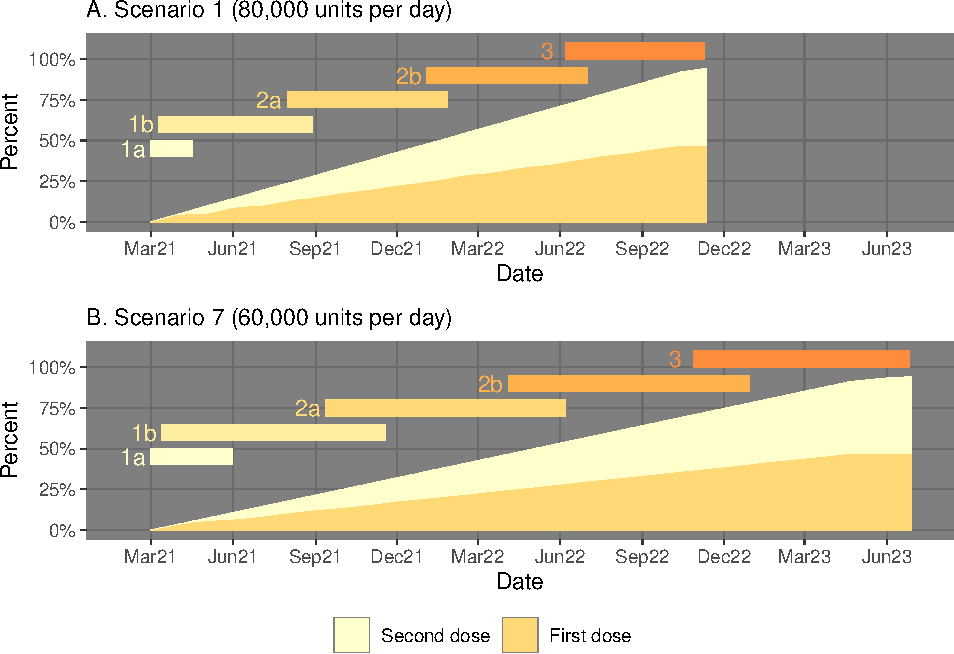
\includegraphics{researchNote_files/figure-latex/unnamed-chunk-4-1.pdf}

\hypertarget{discussion}{%
\section{Discussion}\label{discussion}}

\begin{itemize}
\tightlist
\item
  Don't book your summer holidays just yet.
\end{itemize}

\hypertarget{examples-of-citations-figures-tables-references}{%
\section{Examples of citations, figures, tables,
references}\label{examples-of-citations-figures-tables-references}}

\label{sec:others}

The documentation for \verb+natbib+ may be found at

\begin{center}
  \url{http://mirrors.ctan.org/macros/latex/contrib/natbib/natnotes.pdf}
\end{center}

Of note is the command \verb+\citet+, which produces citations
appropriate for use in inline text. For example,

\begin{verbatim}
   \citet{hasselmo} investigated\dots
\end{verbatim}

produces

\begin{quote}
  Hasselmo, et al.\ (1995) investigated\dots
\end{quote}

\begin{center}
  \url{https://www.ctan.org/pkg/booktabs}
\end{center}

\bibliographystyle{unsrt}
\bibliography{references.bib}


\end{document}
